\documentclass[a4,useAMS,usenatbib]{mn2e}

\usepackage{color}
\usepackage{epsfig}
\usepackage{rotating}
\usepackage{multirow}
\usepackage{amsmath}
\usepackage{amssymb}

%%%%% ASTRO-PH formatting
\setlength{\topmargin}{-0.625in}
\setlength{\oddsidemargin}{-0.25in}
\setlength{\evensidemargin}{-0.25in}

\newcommand*{\chck}[1]{{\color{red}$<$#1$>$}}

\def\degree{$^{\circ}$}
\def\herschel{{\em Herschel}}
\def\spire{\herschel-SPIRE}
\def\higal{Hi-GAL}
\def\pacs{\herschel-PACS}
\def\spitzer{{\em Spitzer}}
\def\mic{$\umu$m}

\title{Milky Way Project : Clouds and Holes Paper}

\author[Simpson et al.]
{\parbox{\textwidth}{R. J. Simpson$^{1}$\thanks{Email: robert.simpson@astro.ox.ac.uk},
C.~J.~Lintott$^{1,2}$,
C.~E.~North$^3$,
and friends...}\vspace{0.8cm}\\
\parbox{\textwidth}{
$^{1}$Oxford Astrophysics, Denys Wilkinson Building, Keble Road, Oxford, OX1 3RH, UK \\
$^{2}$Astronomy Department, Adler Planetarium, 1300 S. Lake Shore Drive, Chicago, IL 60605, USA \\
$^{3}$Department of Physics and Astronomy, Cardiff University, 5 The Parade, Cardiff, CF24 3YB }}


\begin{document}

\date{Accepted 20xx. Received 20xx.}

\pagerange{\pageref{firstpage}--\pageref{lastpage}} \pubyear{2013}

\maketitle

\label{firstpage}

\begin{abstract}
Abstract
\end{abstract}

\section{Introduction}
Infrared dark clouds (IRDCs) were first observed as dark regions
silhouetted against the mid-infrared (MIR) background
\citep{Wilcock2012a} by \emph{Infrared Space Observatory} \citep{ISO}
and \emph{Midcourse Space Experiment} \citep{ISO}. Subsequent
observations showed them to have low temperatures and high densities
($T\lesssim$\,K, $n_H > 10^5$\,cm$^-3$,
e.g.~\citet{Egan98,Carey98,HennebellePerault02}). The IRDC absorbs the
background light and causes a dip in the MIR sky brightness. They are
thought to be the earliest observable formation stages high-mass stars
and stellar clusters.

Following the initial surveys, the MIPSGAL and GLIMPSE surveys used
the IRAC and MIPS instuments on \spitzer allowed the compilation of
larger and more complete catalogues (e.g. \citet{PF09}). With MIR data
alone, however, it is impossible to distinguish this absorption from a
region of inherently lower background emission. Far-Infared (FIR)
observations allow IRDCs, which appear bright at wavelengths above
24\,\mic, to be distinguished from regions of lower emission, which
remain dark -- a 'hole in the sky'
(e.g. \citet{Stanke2010_NGC1999}). It is important to identifying
which of the candidate IRDCs in the catalogues are 'true' dark clouds,
and which are simply holes in the sky. Such interlopers would bias any
statistical studies of IRDCs based on these catalogues.

The HIGAL survey, using the SPIRE and PACS instrument on-board
the \emph{Herschel Space Observatory}, covered a $|b|\le 1\deg$ strip
of the entire Galactic Plane at 70, 160, 250, 350 and 500\,\mic. Using
the 8 and 24\,\mic\ data from GLIMPSE and MIPSGAL, combined with the
longer wavelength data from HIGAL, it is, in princple, possible to
distinguish which objects are clouds and which are holes.

\subsection{Input catalogue}
This study uses candidate IRDCs in the inner regions of the Galactic
Plane (the first and fourth quadrants). We use two catalogues based on
MIR data from the MSX and \spitzer\ surveys (\citet{Simon06,PF09}),
and add to that FIR data from the \herschel HI-GAL survey. The
\citet{Simon06} catalogue (henceforth S06) uses 8\,\mic\ MSX data to
identify over 10000 IRDCs in the region defined by $|l| < 90^{\circ}$
and $|b|<5^{\circ}$. This was restricted to IRDCs greater than 36'' in
size (limited by the 20'' resolution of MSX) and with a sensitivity of
1.2\,MJy/sr. The \citet{PF09} catalogue (henceforth PF09), used
\spitzer\ 8 and 24\,\mic\ data in the region defined by $10^{\circ} <
|l| < 65^{\circ}$ and $|b|<1^{\circ}$. While \spitzer\ data had better
resolution and sensitivity (2'' and 0.3 MJy/sr at 8\,\mic), it covered
a smaller region of the Galactic Plane. The \higal\ survey covers the
full Galactic Plane within $|b|<1^{\circ}$, with a resolution of
$\sim18''$ at 250\,\mic.

Sources included in this study require coverage at both 8 and
24\,\mic. They are selected from PF09, along with sources from S06
which are not within 25'' of a PF09 source. This results in 9931
sources from PF09 (4123 in the range $0 < l < 90$ and 5808 in the
range $270 < l < 360$) and 5731 from S06 (2672 in the range $0 < l <
90$ and 3059 in the range $270 < l < 360$).

\section{Analysis}
Brief outline of analysis

\subsection{Milky Way Project}
The Milky Way Project\footnote{http://www.milkywayproject.org} was established in 2010 as a citizen science interface to data from the \emph{Spitzer} GLIMPSE survey primarily as a search for `bubbles' associated with massive star formation. This effort was successful, and a catalogue of more than 5000 such bubbles which expanded on previous efforts by professional astronomers was published by \citet{Simpsonetal} and used for a statistical analysis of bubble distribution by \citet{Kendrewetal}. Inspired by this success, a second interface was added to the site in order to address the problem of identifying true IRDCs.

As with the previous interface, this new part of the site\footnote{http://www.milkywayproject.org/clouds} makes use of the Zooniverse Application Programming Interface (API) originally built for Galaxy Zoo \citep{Lintottetal} and which supports a large number of similar citizen science projects. This API is primarily responsible for serving images and recording classifications provided by volunteers, who are required to be logged in for their work to be recorded. The interface itself is built in JavaScript and HTML5. Following a short tutorial, an image is selected from the database\footnote{Volunteers see an image they have not yet classified, selected randomly from those with the fewest classifications in the database. This algorithm for task assignment has the advantage of ensuring that images have approximately the same number of classifications at all times, facilitating preliminary data analysis.} and presented to the volunteer who may label it as a \textsc{cloud}, a \textsc{hole} or an \textsc{intermediate} case by selecting one of three buttons, as shown in figure \ref{fig:interface}. Examples of both clouds and holes are provided during the tutorial phase and can be reviewed at any time; these examples are shown in \ref{fig:ex} in both colour schemes available to classifiers. Once an image is classified, the volunteer is shown another image and presented with the opportunity to discuss the first image with other classifiers\footnote{See http://talk.milkywayproject.org}. 

\begin{figure}
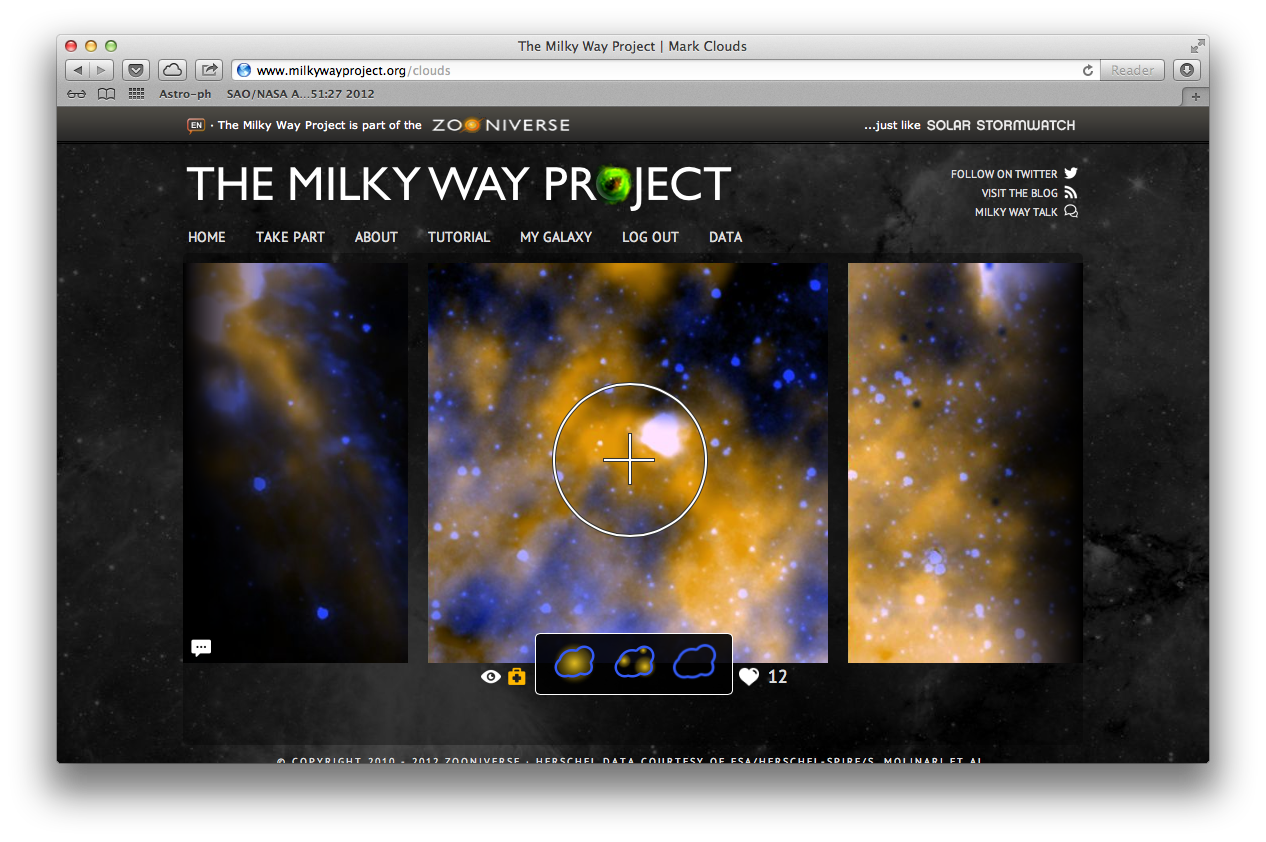
\includegraphics[angle=0,width=0.5\textwidth]{Interface.png}
\caption{The interface for the Clouds part of the Milky Way Project, as seen by classifiers who had to sort each image into one of three categories.}\label{fig:interface}
\end{figure}

DETAILS OF IMAGES AND IMAGE CONSTRUCTION.. Participants can chose to alter the colour palette presented (DO WE RECORD IF PEOPLE USE THIS OPTION?)

\begin{figure}
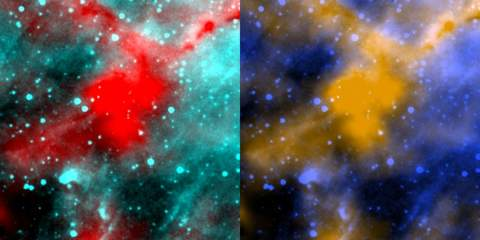
\includegraphics[angle=0,width=0.4\textwidth]{./images/website_examples/cloud1.jpg}
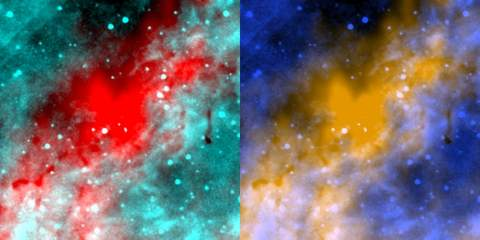
\includegraphics[angle=0,width=0.4\textwidth]{./images/website_examples/cloud2.jpg}
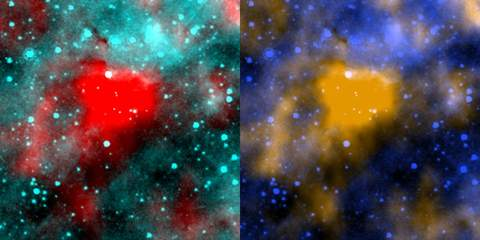
\includegraphics[angle=0,width=0.4\textwidth]{./images/website_examples/cloud3.jpg}
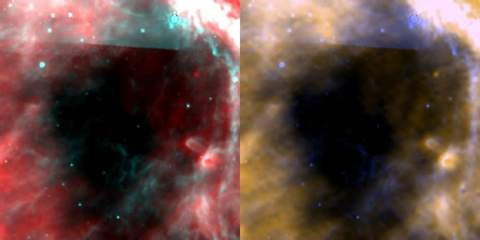
\includegraphics[angle=0,width=0.4\textwidth]{./images/website_examples/hole1.jpg}
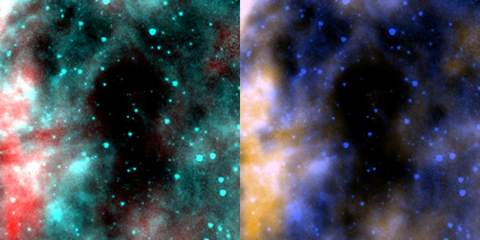
\includegraphics[angle=0,width=0.4\textwidth]{./images/website_examples/hole2.jpg}
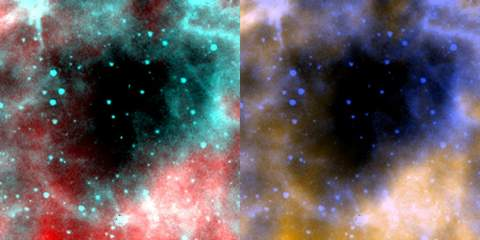
\includegraphics[angle=0,width=0.4\textwidth]{./images/website_examples/hole3.jpg}
\caption{Top three rows : Three of the nine examples of true clouds used in the tutorial. Bottom three rows : Examples of holes given in the tutorial. The tutorial did not include examples of 'intermediate' images.}\label{fig:ex}
\end{figure}


The clouds project was launched on XXXXXXX and ran until XXXXXXX, collecting 1.1 million classifications. 3544 logged-in users provided classifications. However, approximately half of the classifications were received from those who were not logged in. The most active user has completed 59020 classifications and is one of three users to have seen every image provided. (HOW DO WE HANDLE THE REPEATS IN DATA REDUCTION). 3253 classifiers provided more than five classifications (91.9\%, compared to 25\% in the previous incarnation of the Milky Way Project), 1843 more than fifty (52.0\% compared to 5.7\%) and 168 five hundred classifications or more. 

DETAILS OF NON-LOGGED IN USERS


MWP interface and initial results (or in results section?)
User and classification numbers and duration of dataset used

Raw classifications?
Histogram of results?


\subsection{Experts and Training data}

In order to turn the more than one million classifications into a useful scientific catalogue, it is necessary to determine consensus classifications. This process typically involves assigning a weight to each classifier based on their behaviour. For example, the weighting scheme in \citet{Lintott} rewards those who agree with the consensus, minimizing the effect of extreme or erratic classifiers, while \citet{Schwamb} use synthetic data to provide an objective measure of classifier performance. The Milky Way Project bubble catalogue described in \citet{Simpson} used user behaviour on the site as a strong indication of expertise, discarding classifications from those who, for example, only ever marked circular rather than elliptical bubbles. 

This paper introduces a generalized approach to user weighting based on performance against a set of expert-classified `gold standard' data, described below. Images with expert data available were presented randomly alongside the rest of the dataset. However, because of the high mean number of classifications per user it is possible for this project to use an approach in which only those who have seen such images have adjusted weightings. This avoids the complication of requiring an iterative approach to user weightings (as in \citet{Lintott} and \citet{Schwamb}) and allows us to take into account changes in user accuracy over time. Such changes are expected to be significant, particularly at the start of a volunteer's classification career (see \citet{EdwinSimpson} for a discussion of citizen science user trajectories). 

To generate a gold standard dataset a naive consensus for each image (in which all classifiers are treated equally) was first calculated. Those images which had the highest votes in each category (\textsc{cloud}, \textsc{intermediate} or \textsc{hole}) were inspected by one of the authors (RS) with correctly classified images being retained. In all, XXXXX of each type were included, and a list of those sources included in the training sets is given in table \ref{tab:gold}. 

\begin{table}
\begin{tabular}{|c|c|c|}
\hline
\textsc{cloud} & \textsc{intermediate} & \textsc{hole}\\
\hline
Source ID & Source ID & Source ID\\
\hline
\end{tabular}
\caption{List of sources in the `gold standard' training set for each of the three categories}\label{tab:gold}
\end{table}

Definition of training data definition

Thumbnails of training data and classifications

Expert versus general results (plot)

\subsection{Analysis sequence}

The presence of an intermediate category into which images can be sorted raises questions of interpretation. It is not intended to represent a separate category of object which is in some sense truly intermediate between an IRDC and a `hole', but rather the situation where it is difficult (or impossible) to distinguish between the two extreme cases. We can think of the situation in terms of probabilities; a classifier choosing the `cloud' button is asserting that the probability that the object being classified is, or is close to, 1. Viewed this way, a classifier choosing the `intermediate' classification is asserting that the image does not allow them to make a judgement about the probability the image represents a cloud. In such circumstances, a valid choice is to maintain our prior assessment of the probability, typically (in the absence of other classifications, p=0.5 is chosen). 

In order to be able to assess the effect of the intermediate category, we first use only classifications from the other two buttons. This leaves XXXXXX, roughly two-thirds of the original classifications. 

[HOW UNEVEN WERE THE INTERMEDIATE CLASSIFICATIONS OVER SUBJECTS]




\subsubsection{Notes from 15th August}

All the 1.1 million classifications are run through sequentially in time.

Issues caused because users have three options - cloud, hole or intermediate. (see GZ argument about non-classified galaxies). All clouds start with an initial score of 0.5, which is updated based on the user's skill level. Skill level is determined by users encountering training data. 

Note that the tutorial doesn't really say much about intermediates - or at least it only says the button exists. We should therefore expect a wide range of user behaviours - including those who use it as a `don't know' alongside those who genuinely only use it for intermediate. This means that weighting is important for this category (?). 

How do we treat the intermediate classifications? 

	Option A : A third genuine category - therefore need expert data with all three classifications in order to distinguish between the confused and those who are classifying something as intermediate. Cuts are needed for each population producing three lists (which might overlap). 
	
	Option B : Treat cloud to hole as a continuous distribution where somethings are definitely (p=1) clouds, some definitely (p=0) holes but most lie somewhere in between. In this model intermediate votes signify p=0.5. In other words we're forcing a discrete estimate of probability.This produces a catalogue including all the objects with the best value probability for each one to which thresholds can be applied. 
	
	(Option C : Ignore the intermediate classifications) We might want to test the effect of adding the intermediate button). 
	
	Possible changes to training set :
	
		i. Add a set of `definite' intermediate objects reviewed by experts as existing set. Give these the `correct' value of 0.5 and adjust user skill levels accordingly.
		
		ii. Get N experts to classify - award 1 for cloud, 0.5 for intermediate, 0 for hole, take average - adjust user skill level for being close to the average. Close to be defined (might want N to be even so 0.5 can be a `correct' answer). 
		
		iii. Get expert assign numerical value (e.g. 0.7). This won't work as people - even experts - are crap at this (and because it's not really a linear continuous scale). 

The procedure
Growth charts
Results of MC runs
Any threshholds


\section{Results}
Results from analyis (cloudiness chart)

Histogram of classifications before \& after

Thumnail examples of clouds, holes and unknowns

Full table of results

\section{Conclusions}


\section{Acknowledgements}
This publication has been made possible by the participation of more than 40,000 volunteers on the Milky Way Project. Their contributions are acknowledged individually at http://www.milkywayproject.org/authors. The Milky Way Project, and R.J.S. were supported by The Leverhulme Trust. Development of the MWP was partly supported by the National Science Foundation CDI grant: DRL-0941610. 

This work is based on observations made with the Spitzer Space Telescope, which is operated by the Jet Propulsion Laboratory, California Institute of Technology under a contract with NASA. This research has made use of the SIMBAD database, operated at CDS, Strasbourg, France.

{\em Herschel} is an ESA space observatory with science instruments
provided by European-led Principal Investigator consortia and with important
participation from NASA.

SPIRE has been developed by a consortium of institutes led by Cardiff
Univ. (UK) and including: Univ. Lethbridge (Canada); NAOC (China);
CEA, LAM (France); IFSI, Univ. Padua (Italy); IAC (Spain); Stockholm
Observatory (Sweden); Imperial College London, RAL, UCL-MSSL, UKATC,
Univ. Sussex (UK); and Caltech, JPL, NHSC, Univ. Colorado (USA). This
development has been supported by national funding agencies: CSA
(Canada); NAOC (China); CEA, CNES, CNRS (France); ASI (Italy); MCINN
(Spain); SNSB (Sweden); STFC, UKSA (UK); and NASA (USA).

This research made use of APLpy, an open-source plotting package for
Python hosted at http://aplpy.github.com

\bibliographystyle{mn2e}
\bibliography{Clouds_bibCN}

\end{document}
